\section{Appendice}
\subsection{Ciclo di Deming}
Alla luce delle informazioni sopra citate il team ha deciso di adottare la politica del ciclo PDCA per le attivit\'a da svolgere. Lo stesso, oltre a fornire supporto nella pianificazione garantisce un elevato standard qualitativo tramite il \textit{Miglioramento continuo}, che è alla base del ciclo di Deming.
\begin{figure}[H]
\centering
     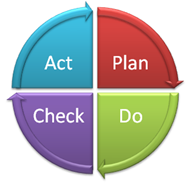
\includegraphics[scale=1]{../modello/img/pdca}\\
     \caption{Ciclo di Deming}\label{fig:1}
\end{figure}
\begin{itemize}
\item \textbf{\textit{Plan}}: pianificazione che prevede la definizione di procedure, risorse, scadenze e responsabilit\'a ;
\item \textbf{\textit{Do}}: esecuzione delle attivit\'a pianificate; 
\item \textbf{\textit{Check}}: controllo dei risultati ottenuti e confronto con quelli pianificati;
\item \textbf{\textit{Act}}: Analisi dei risultati ottenuti e modifica o definizione di nuove procedure che permettano di evitare gli aspetti critici dei processi in esame.
\end{itemize}
L'adozione del PDCA garantisce un continuo arricchimento dei processi tramite dei cambiamenti e delle riorganizzazioni. Alla base di questo, ci deve essere una conoscenza specifica delle \infoNDP{} da parte di tutti i componenti del team. Inoltre, queste migliorie aumentano i costi di gestione e per questo devono essere valutati dal \textit{Responsabile di progetto}.
\subsection{ISO/IEC 9126}
Lo standard ISO/IEC 9126 descrive gli obiettivi qualitativi di prodotto e delinea in generale le metriche per misurare il raggiungimento di tale obiettivo (figura 3). In questo standard i criteri sono divisi in 3 aree diverse:
\begin{figure} [H]
\centering
     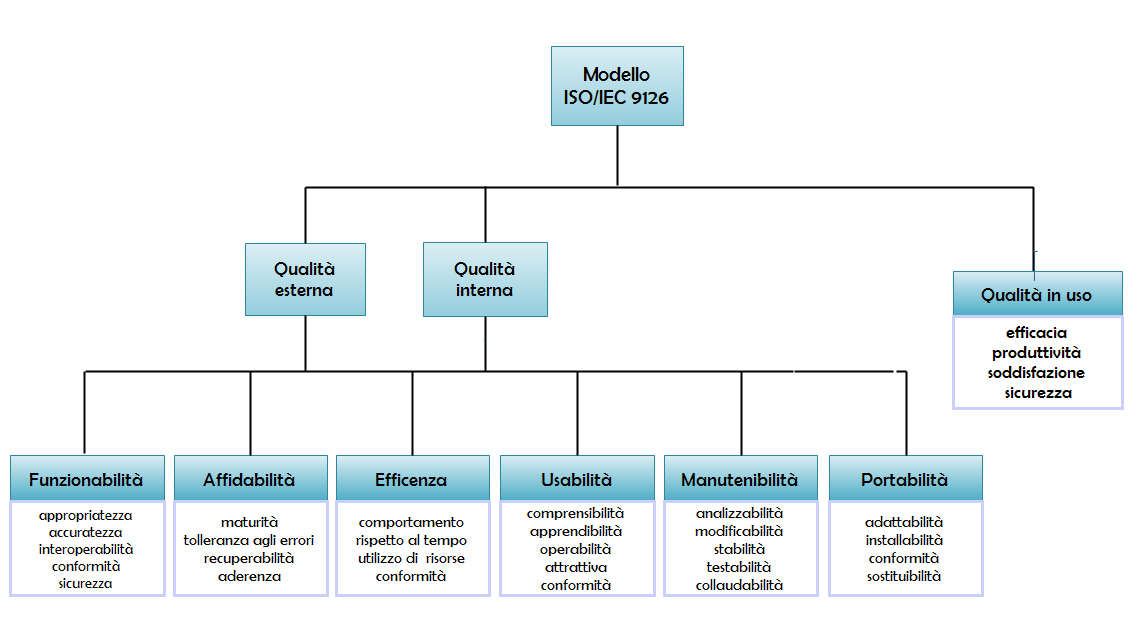
\includegraphics[scale=0.5]{../modello/img/iso9126}\\
     \caption{Caratteristiche qualitative definite dal modello ISO/IEC 9126}\label{fig:3}
\end{figure}
\begin{itemize}
\item \textbf{Qualit\'a in uso}:\'e la qualit\'a del software dal punto di vista dell'utilizzatore;
\item \textbf{Qualit\'a esterna}:\'e la qualit'a del software dal punto di vista esterno nel momento in cui esso viene eseguito e testato in ambiente di prova;
\item \textbf{Qualit\'a interna}:\'e la qualit\'a del software vista dall'interno e quindi sono le caratteristiche implementative del software quali architettura e codice che ne deriva.
\end{itemize}
Non avendo modo di verificare la qualit\'a in uso, \gruppo ha deciso di lavorare su qualit\'a interna ed esterna definendo apposite metriche.
\begin{itemize}
\item \textbf{Funzionalit\'a} \'e la capacità di un prodotto software di fornire funzioni che soddisfano esigenze stabilite, necessarie per operare sotto condizioni specifiche.
\begin{itemize}
\item Appropriatezza: rappresenta la capacità del prodotto software di fornire un appropriato insieme di funzioni per gli specificati compiti ed obiettivi prefissati all'utente.
\item Accuratezza: la capacità del prodotto software di fornire i risultati concordati o i precisi effetti richiesti;
\item Interoperabilità: è la capacità del prodotto software di interagire ed operare con uno o più sistemi specificati;
\item Conformità: la capacità del prodotto software di aderire a standard, convenzioni e regolamentazioni rilevanti al settore operativo a cui vengono applicate;
\item Sicurezza: la capacit\'a del prodotto software di proteggere informazioni e dati negando in ogni modo che persone o sistemi non autorizzati possano accedervi o modificarli, e che a persone o sistemi effettivamente autorizzati non sia negato l’accesso ad essi.
\end{itemize}
\item \textbf{Affidabilit\'a}: \'e la capacità del prodotto software di mantenere uno specificato livello di prestazioni quando usato in date condizioni per un dato periodo.
\begin{itemize}
\item Maturità: \'e la capacità di un prodotto software di evitare che si verificano errori, malfunzionamenti o siano prodotti risultati non corretti;
\item Tolleranza agli errori: \'e la capacità di mantenere livelli predeterminati di prestazioni anche in presenza di malfunzionamenti o usi scorretti del prodotto;
\item Recuperabilità: \'e la capacità di un prodotto di ripristinare il livello appropriato di prestazioni e di recupero delle informazioni rilevanti, in seguito a un malfunzionamento. A seguito di un errore, il software può risultare non accessibile per un determinato periodo di tempo, questo arco di tempo \'e valutato proprio dalla caratteristica di recuperabilità;
\item Aderenza: è la capacità di aderire a standard, regole e convenzioni inerenti all'affidabilità.
\end{itemize}
\item \textbf{Usabilit\'a}: \'e la capacità del prodotto software di essere capito, appreso, usato e benaccetto dall'utente, quando usato sotto condizioni specificate.
ottimale”
\begin{itemize}
\item Comprensibilità: esprime la facilità di comprensione dei concetti del prodotto, mettendo in grado l'utente di comprendere se il software è appropriato.
\item Apprendibilità: è la capacità di ridurre l’ impegno richiesto agli utenti per imparare ad usare la sua applicazione;
\item Operabilità: è la capacità di mettere in condizione gli utenti di farne uso per i propri scopi e controllarne l’uso;
\item Attrattiva: è la capacità del software di essere piacevole per l'utente che ne fa uso;
\item Conformità: è la capacità del software di aderire a standard o convenzioni relativi all'usabilità.
\end{itemize}
\item \textbf{Efficienza}: \'e la capacità di fornire appropriate prestazioni relativamente alla quantità di risorse usate.
\begin{itemize}
\item Comportamento rispetto al tempo: è la capacità di fornire adeguati tempi di risposta, elaborazione e velocità di attraversamento, sotto condizioni determinate;
\item Utilizzo delle risorse: è la capacità di utilizzo di quantità e tipo di risorse in maniera adeguata.
\item Conformità: è la capacità di aderire a standard e specifiche sull'efficienza\ped{G}.
\end{itemize}
\item \textbf{Manutenibilit\'a}: \'e la capacità del software di essere modificato, includendo correzioni, miglioramenti o adattamenti.
\begin{itemize}
\item Analizzabilità: rappresenta la facilità con la quale è possibile analizzare il codice per localizzare un errore nello stesso;
\item Modificabilità: la capacità del prodotto software di permettere l'implementazione di una specificata modifica (sostituzioni componenti);
\item Stabilità: la capacità del software di evitare effetti inaspettati derivanti da modifiche errate;
\item Testabilità: la capacità di essere facilmente testato per validare le modifiche apportate al software.
\end{itemize}
\item \textbf{Portabilit\'a}: \'e la capacità del software di essere trasportato da un ambiente di lavoro ad un altro.
\begin{itemize}
\item Adattabilità: la capacità del software di essere adattato per differenti ambienti operativi senza dover applicare modifiche diverse da quelle fornite per il software considerato;
\item Installabilit\'a: la capacità del software di essere installato in uno specificato ambiente;
\item Conformit\'a: la capacità del prodotto software di aderire a standard e convenzioni relative alla portabilità;
\item Sostituibilit\'a: è la capacità di essere utilizzato al posto di un altro software per svolgere gli stessi compiti nello stesso.
\end{itemize}
\end{itemize}
\subsection{Capability Maturity Model Integration (CMMI)}
\begin{figure} [H]
\centering
     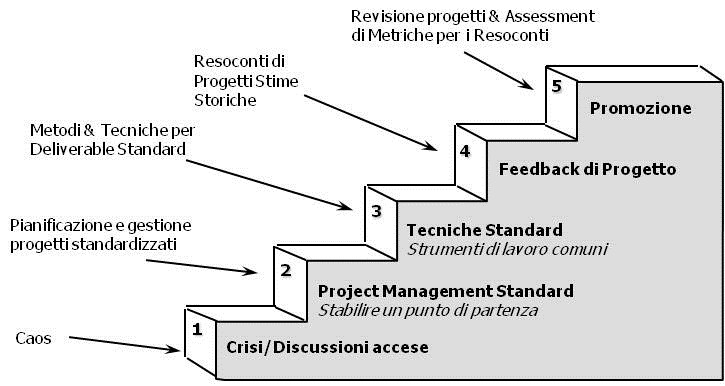
\includegraphics[scale=0.8]{../modello/img/CMMI}\\
     \caption{Livello di maturit\'a delle procedure}\label{fig:2}
\end{figure}
Il modello identifica cinque livelli di maturità dei processi all'interno di un'organizzazione: dal Livello 1, il processo\ped{G} più immaturo, o caotico, al Livello 5, il processo\ped{G} più maturo, o di qualità
\begin{itemize}
\item \textbf{Livello di maturità 1}\\
Partendo dall'assunzione che una pratica non può essere migliorata se non è ripetibile, il livello di maturità iniziale vede l'organizzazione effettuare la gestione delle persone tramite procedure ad hoc, spesso informali e non ripetibili se non sporadicamente. Un esempio tipico è data dall'impossibilità, da parte delle persone, di assicurare la data di rilascio del software, indipendentemente dalle tecnologie utilizzate o dalla preparazione delle persone. Un'altra conseguenza tipica è la gestione incontrollata delle modifiche ai requisiti con conseguenze negative sui piani di lavoro.
L'attività principale da compiere in questa fase è quella di aiutare l'organizzazione a rimuovere ogni impedimento alla ripetibilit\`a delle pratiche;
\item \textbf{Livello di maturità 2}\\
Al livello di maturità 2, l'organizzazione stabilisce una politica per divulgare presso tutti i gruppi di lavoro i processi stabiliti. Prima di pensare ad ogni miglioramento, l'organizzazione deve assicurare un ambiente di lavoro stabile in cui eseguire in maniera ripetibile i propri processi. Finché si opera in una modalità non strutturata, il management è troppo occupato nel controllo quotidiano delle operazione per poter pensare a qualsivoglia cambiamento in ottica di miglioramento. L'obiettivo principale del livello 2 è quindi quello di permettere alle persone di svolgere il proprio lavoro in maniera ripetibile, in base a quanto già fatto in passato ed in base all'esperienza maturata. A questo livello il management lascia ai responsabili dei singoli gruppi il compito di controllare il lavoro quotidiano, dedicandosi a sua volta al controllo dei risultati finali e della baseline (ed alle rispettive modifiche).
Solo quando le pratiche stabilite saranno eseguire con naturalezza dall'intera organizzazione, questa potrà iniziare la fase successiva di utilizzo di processi comuni a tutta l'organizzazione;
\item \textbf{Livello di maturità 3}\\
Al livello di maturità 3, l'organizzazione seleziona le migliori pratiche e le include in un processo comune. Operando tutti con le stesse pratiche definite, l'organizzazione sarà in grado di valutare le pratiche con migliori performance nell'ambiente comune. Documentate nell'ambito del processo comune le pratiche, queste diventano anche lo strumento di apprendimento per le nuove persone. Le misure effettuate sulle pratiche di maggiore criticità sono registrate in un archivio ed utilizzare per effettuarne l'analisi.
In tale modo si è creato il fondamento per una cultura di base comune all'organizzazione: un processo comune conosciuto ed applicato da tutti. E' il fondamento della cultura professionale di base dell'organizzazione;
\item \textbf{Livello di maturità 4}\\
Al livello di maturità 4, l'organizzazione inizia a gestire i processi in base ai risultati utilizzando l'analisi delle misure effettuate. Le attività sono svolte secondo i processi comuni definiti ed i risultati sono quindi più controllabili in base all'esperienza storica. Le deviazioni dai risultati attesi sono analizzate, le cause delle deviazioni individuate e le azioni correttive prese di conseguenza.
I processi sono quindi gestiti quantitativamente ed i risultati sono prevedibili con maggiore cura. I risultati del business sono controllati da valori e non più dalle \textit{milestone\ped{G}} come prima. Si crea quindi la cultura per un vero miglioramento dei processi e quindi delle performance reali;
\item \textbf{Livello di maturità 5}\\
Al livello di maturità 5, l'organizzazione opera utilizzando in maniera ripetitiva i propri processi, ne valuta le performance quantitativamente ed opera per migliorarli di continuo. Gli eventuali difetti sono analizzati e le cause che li generano sono rimosse per evitare il loro ripetersi.
Le persone sono culturalmente abituate ad eseguire i processi conosciuti ed il management a gestirli quantitativamente ed a migliorarli. Si crea anche la cultura dell'accettazione del cambiamento. L'organizzazione entra in un circolo virtuoso di miglioramento continuo;
\end{itemize}
